\subsection{Consideraciones generales}
 

\subsection{Circuito Derivador}
Para armar los circuitos propuestos por la cátedra se dispone de un
amplificador operacional LM-833N. Los datos más importantes a considerar
vistos en la hoja de datos son los siguientes:
\begin{itemize}
    \item $A_{vol}$ = $110dB$ 
    \item BWP = $15 MHz$
    \item $\omega_b$ = $47 Hz$
\end{itemize}   

A continuación, se realiza el análisis sobre el circuito derivador planteado
por la cátedra utilizando un amplificador operacional $LM833$ aplicado en el siguiente circuito.
\begin{figure}[H]
    \centering
    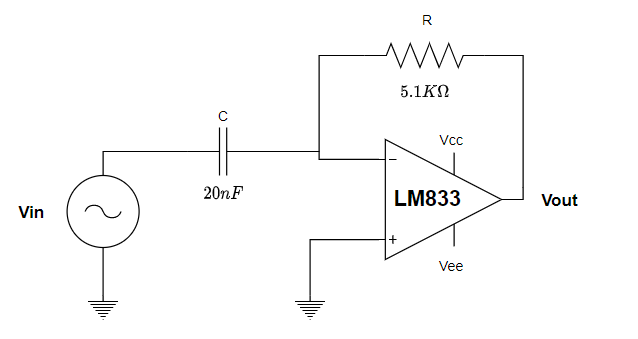
\includegraphics[width=0.6\textwidth]{../Ejercicio3-CircuitoIntegradoresyDerivadores/Imagenes/Derivador/circuito_derivador.png}
    \caption{Circuito derivador implementado con Opamp}
\end{figure}
Se obtuvo una diferencia entre los valores teóricos y medidos de los componentes 
que se muestran en la siguiente tabla.
\begin{table}[H]
    \centering
    \begin{tabular}{|c|c|c|}
    \hline
                 & C       & R             \\ \hline
    Teórcio      & 20 nF   & 5k1$\Omega$   \\ \hline
    Medido       & 18.8 nF & 5.27 $\Omega$ \\ \hline
    $\epsilon_r$ & 6.4\%    & 3.3\%          \\ \hline
    \end{tabular}
    \end{table}


\subsubsection{Respuesta en frecuencia}
Consiguientemente, se procede a calcular la transferencia de tensión entra
la entrada y salida del circuito. \par 
En condición ideales, se considera que la ganancia del
amplificador operacional es infinita, por lo que, basándonos en 
su ecuación característica (\ref{eq_opamp}), se puede asegurar que para 
mantener la relación $V^+=V^-$, la resta entre ambos voltajes va a tender a 0.
\vspace{2mm}
\begin{equation}
    V_{out}=A_0(V^+-V^-)  \rightarrow V_{out}=-A_0V^-
    \label{eq_opamp}
\end{equation}
\vspace{2mm}
Por lo tanto, se pueden escribir a las corrientes del circuito como:
\vspace{2mm}
\begin{equation}
    I_1=\frac{V{in}}{X_c}=V_{in}\$C_1 \indent \indent I_2=\frac{V_{out}}{R}
    \label{eq_avol_ideal}
\end{equation}
\vspace{2mm}
Considerando que $V^-=0$ y que $I_1=I_2$ se logra llegar a la transferencia bajo 
condiciones ideales:
\vspace{2mm}
\begin{equation}
    H(\$)=\frac{V_{out}}{V_{in}}=-R\$C
    \label{trans_ideal}
\end{equation}
\vspace{2mm}
Por otro lado, considerando a $A_{vol}$ finito se vuelve indispensable reformular las
ecuaciones vistas en \ref{eq_avol_ideal} ya que al considerar un $A_{vol}$ que no 
tiende a infinito se vuelve imposible asegurar que la tensión $V^-$ sea nula. Bajo 
las nuevas circunstancias se obtienen:
\vspace{2mm}
\begin{equation}
    I_1=\frac{V{in}-V^-}{X_c}=(V_{in}-V^-)\$C_1 \indent \indent I_2=\frac{V_{out}-V^-}{R}
    \label{eq_avol_noideal}
\end{equation}
\vspace{2mm}
Utilizando \ref{eq_opamp} y \ref{eq_avol_noideal} se puede despejar la transferencia
como:
\vspace{2mm}
\begin{equation}
    H_1(\$)=\frac{V_{out}}{V_{in}}=\frac{-R\$C}{1+\left(\frac{R\$C+1}{A_0}\right)}=- \left(\frac{A_{vol}RC}{A_{vol}+1}\right)\frac{\$}{ \left(\frac{\$}{\frac{A_{vol}+1}{RC}}\right)+1}
    \label{trans_no_ideal}
\end{equation}
\vspace{2mm}
Se puede validar este ecuación considerando:
 $$\lim_{A_0\to\infty} H_1(\$)=H(\$)$$
Obteniéndose la transferencia en condiciones ideales vista en \ref{trans_ideal}. \par
Para finalizar se realiza un análisis considerando $A_{vol}$ variante en frecuencia
debido a la presencia de un polo dominante que le da una respuesta en frecuencia 
característica de un filtro pasa-bajos. La dependencia en frecuencia de la ganancia
del opamp está dada por la siguiente fórmula:
\vspace{2mm}
\begin{equation}
    A_v(\$)=\frac{A_0}{1+\frac{\$}{w_b}}
    \label{a_vol_frec}
\end{equation}
\vspace{2mm}
Siendo $A_0$ la ganancia en lazo abierto del opamp y $w_b$ la frecuencia del polo dominante,
 frecuencia para la cual el dispositivo atenúa 3 dB. \par 
 Reemplazando (\ref{a_vol_frec}) en (\ref{trans_no_ideal}) se obtiene:
 \vspace{2mm}
 \begin{equation}
    H_2(\$)=\frac{-R\$C}{\left(1+\frac{1}{A_0}\right)+\$\left(\frac{RCw_b+1}{w_bA_0}\right)+\frac{\$^2}{\frac{w_bA_0}{RC}}}
    \label{trans_frec}
\end{equation}
\vspace{2mm}
Esta ecuación se puede dividir según su ganancia ideal $G_I$ y su factor de corrección
$F_c$ de la siguiente forma:
\vspace{2mm}
\begin{equation*}
   G_I=-R\$C \indent \indent F_c={\left(1+\frac{1}{A_0}\right)+\frac{\$(RCw_b+1)}{w_bA_0}+\frac{R\$^2C}{w_bA_0}}
   \label{trans_frec}
\end{equation*}
\vspace{2mm}
Siguiendo el mismo procedimiento aplicado para $H_1(\$)$, se puede formular:
 $$\lim_{A_0\to\infty} H_2(\$)=\lim_{A_0\to\infty} G_IF_C=G_I=H(\$)$$

Las expresiones obtenidas se plasman en el siguiente gráfico, pudiéndose 
observar una mayor precisión a medida que se usan modelos más realistas
sin consideraciones ideales.

\begin{figure}[H]
    \centering
    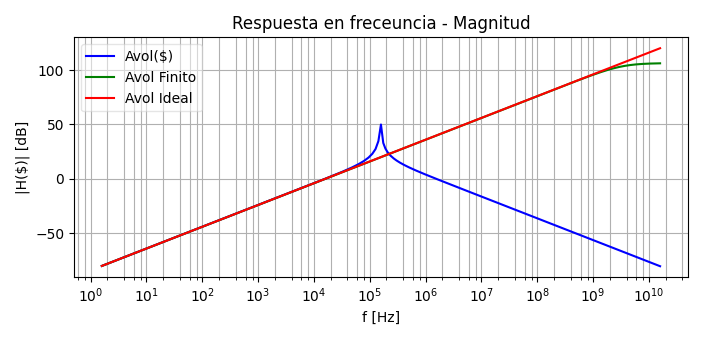
\includegraphics[width=0.6\textwidth]{../Ejercicio3-CircuitoIntegradoresyDerivadores/Imagenes/Derivador/bode_derivador_magnitud.png}
    \caption{Respuesta en frecuencia teóricas - Módulo}
\end{figure}
\begin{figure}[H]
    \centering
    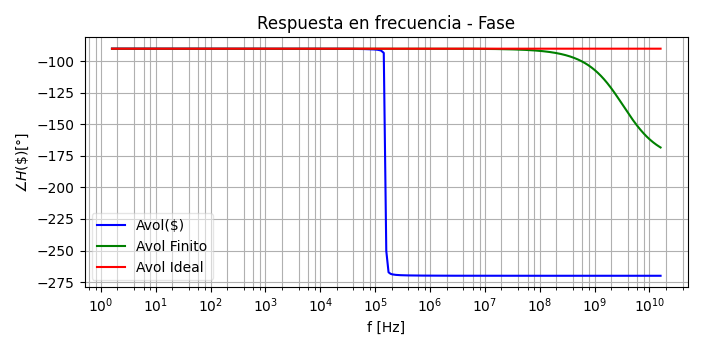
\includegraphics[width=0.6\textwidth]{../Ejercicio3-CircuitoIntegradoresyDerivadores/Imagenes/Derivador/bode_derivador_fase.png}
    \caption{Respuesta en frecuencia teóricas - Fase}
\end{figure}

A mayores frecuencias se puede observar un par de polos conjugados en el modelo de 
$A_{vol}$ finito, cuya frecuencia se puede despejar de la función transferencia \ref{trans_frec}, tomando 
la misma el siguiente valor:
\begin{equation}
    \vspace{2mm}
    f_0=\frac{1}{2\pi}\sqrt{\frac{w_b(A_0+1)}{RC}}\approx 154.5KHz
    \vspace{2mm}
\end{equation}
Por otro lado, al considerar que el sobrepico presente es de magnitud considerable
y que el cambio de fase es rápido, se esperara un $\xi$ relativamente bajo que 
indique un circuito sumamente subamortiguado. Dicho valor se puede despejar
de  \ref{trans_frec} como el valor anterior:
\begin{equation}
    \vspace{2mm}
    \xi=\frac{w_0(RCw_b+1)}{2A_0w_b}\approx \num{5.22e-3}
    \vspace{2mm}
\end{equation}
Tomando en consideración $A{vol}$ finito, se observa la transferencia hallada 
en \ref{trans_no_ideal}. De la misma se desprende la presencia de un polo en:
\begin{equation}
    \vspace{2mm}
    f=\frac{A{vol}+1}{RC}\approx 508MHz
    \vspace{2mm}
\end{equation}
Esto coincide con lo visto en el gráfico ya que aproximadamente una década por 
debajo empieza un desfasaje de -90$^\circ$ que termina una década por encima.
Bajo lo anteriormente expuesto, los cálculos despejados de la ecuación coinciden
con lo visto en los gráficos. A fines prácticos, dicho polo no es de interés 
ya que el circuito no será utilizados a altas frecuencias.\par 
A continuación, se presentan la respuesta en frecuencia tanto simulada como medida 
en el circuito.


\begin{figure}[H]
    \centering
    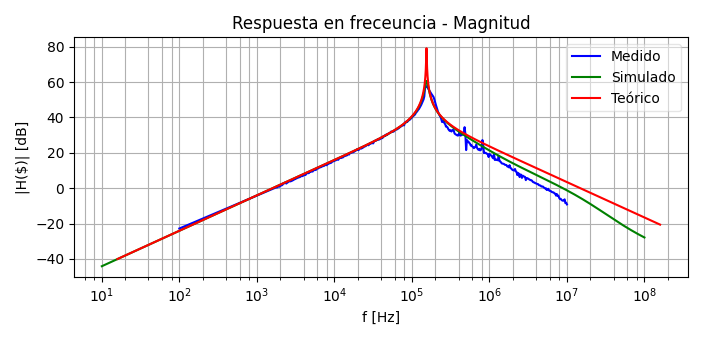
\includegraphics[width=0.6\textwidth]{../Ejercicio3-CircuitoIntegradoresyDerivadores/Imagenes/Derivador/comparacion_magnitud.png}
    \caption{Comparación respuesta en frecuencia - Módulo}
    \label{graph_trans_mag}
\end{figure}
\begin{figure}[H]
    \centering
    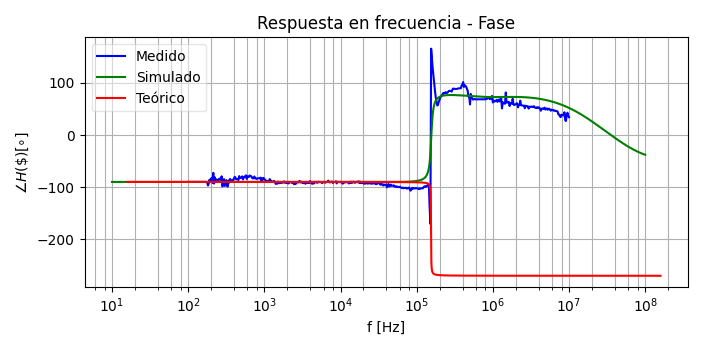
\includegraphics[width=0.6\textwidth]{../Ejercicio3-CircuitoIntegradoresyDerivadores/Imagenes/Derivador/comparacion_fase.png}
    \caption{Comparación respuesta en frecuencia - Fase}
    \label{graph_trans_pha}
\end{figure}
Observando las figuras anteriores, se hace presente una correcta correlación entre
el modelo teórico, la experiencia simulada y su realización empírica.
Al ser de interés su comportamiento como derivador el circuito tendrá que ser usado a una 
frecuencia inferior a los $100 KHz$, frecuencias para las cuales el comportamiento es 
consistente para los tres casos. \par 

Consideramos pertinente comentar los problemas presentes al intentar medir el sobrepico de la respuesta en frecuencia
debido a que el equipo \textit{Electronic Explorer} realiza el barrido en frecuencia usando una señal de entrada configurable
de un $1V$, la cual al estar en el pico, es amplificada en más de $40dB$. Dicha amplificación
nos producía que el sistema se fuera de escala, siendo imposible 
detectarlo. Por otro lado, al experimentar con una tensión de entrada menor, la señal ya se perdía junto con
el ruido  de alta frecuencia presente en el sistema. \par  Para sortear dicho problema
se implementó el circuito mostrado en \ref{circuito_medidor_derivador}, utilizando un atenuador de $40dB$ más un buffer,
de manera tal de separar las etapas y que no se carguen entre si. De esta manera, se logró medir efectivamente el pico 
postulado tanto en el modelo simulado como el teórico.

\begin{figure}[H]
    \centering
    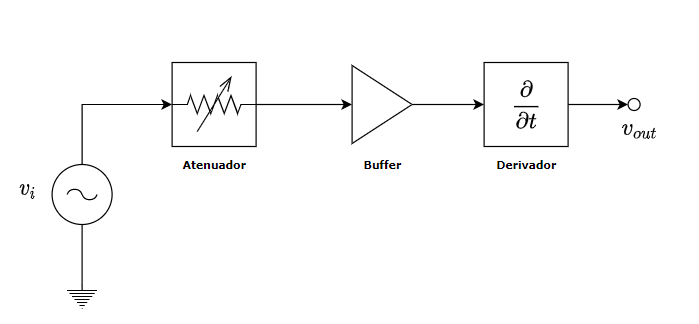
\includegraphics[width=0.6\textwidth]{../Ejercicio3-CircuitoIntegradoresyDerivadores/Imagenes/Derivador/circuito_medidor.png}
    \caption{Circuito de medición para la respuesta en frecuencia}
    \label{circuito_medidor_derivador}
\end{figure}



\subsubsection{Impedancia de entrada}

Para calcular la impedancia de entrada se procede con el mismo análisis que para 
la transferencia, considerando los distintos modelos para la ganancia del opamp. Para el primer 
caso, el hecho de poseer una $A_{vol}$ de carácter infinito induce una tierra virtual 
perfecta en $V^-$, permitiendo llegar a:

\vspace{2mm}
\begin{equation}
   Z_{in_1}=\frac{V_i}{I_1}=\frac{1}{\$C} 
    \label{zin_ideal}
\end{equation}
\vspace{2mm}
Por otro lado, al considerar una ganancia finita, se puede despejar de \ref{eq_avol_noideal} y \ref{eq_opamp}
la impedancia de entrada para el caso no ideal.

\vspace{2mm}
\begin{equation}
    Z_{in2}=\frac{V_i}{I_1}=\frac{1}{\$C}\frac{1}{\left(1-\frac{R\$C}{1+A_0+R\$C}\right)} 
    \label{zin_avol_ideal}
\end{equation}
\vspace{2mm}

Se puede validar este ecuación considerando:
 $$\lim_{A_0\to\infty} Z_{in_2}=Z_{in_1}$$
Para finalizar, se reemplaza la variación en frecuencia del opamp dada por \ref{a_vol_frec}, obteniéndose:

\vspace{2mm}
\begin{equation}
    Z_{in3}=\frac{V_i}{I_1}=\frac{1}{\$C}\frac{1}{1-\frac{R\$C+\frac{R\$^2C}{w_b}}{\frac{R\$^2C}{w_b} +\$(RC+\frac{1}{w_b})+(1+A_0)}} 
    \label{zin_avol_frec}
\end{equation}
\vspace{2mm}

También, se puede validar este ecuación considerando:
 $$\lim_{A_0\to\infty} Z_{in_3}=Z_{in_1}$$

Las expresiones obtenidas se plasman en el siguiente gráfico, pudiéndose 
observar una mayor precisión a medida que se usan modelos más realistas
sin consideraciones ideales.

\begin{figure}[H]
    \centering
    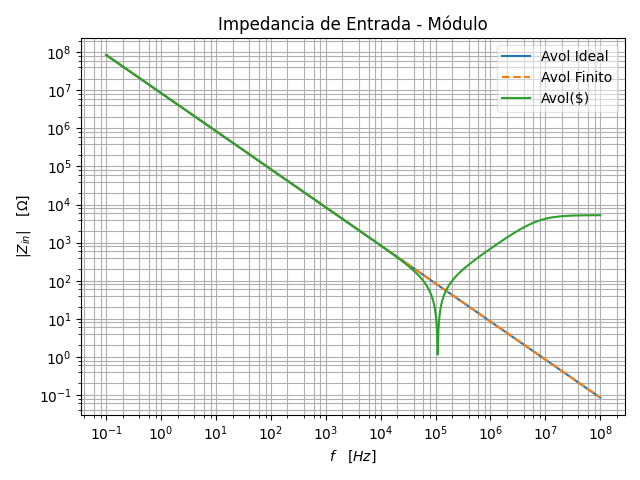
\includegraphics[width=0.6\textwidth]{../Ejercicio3-CircuitoIntegradoresyDerivadores/Imagenes/Derivador/Zin/impedancia_teo_mag.png}
    \caption{Impedancias de entrada teóricas - Módulo}
\end{figure}
\begin{figure}[H]
    \centering    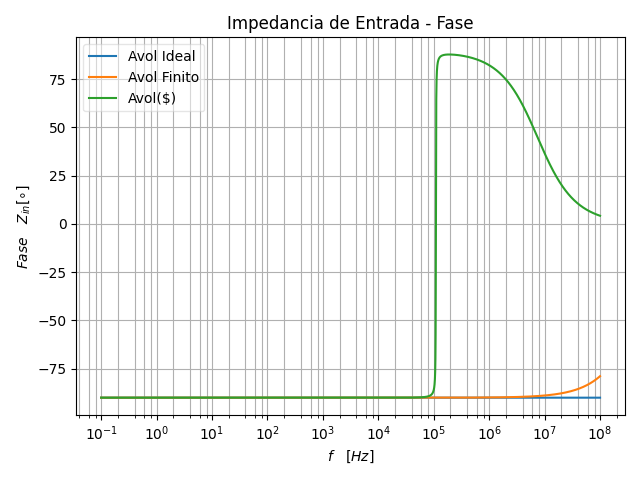
\includegraphics[width=0.6\textwidth]{../Ejercicio3-CircuitoIntegradoresyDerivadores/Imagenes/Derivador/Zin/impedancia_teo_fase.png}
    \caption{Impedancias de entrada teóricas - Fase}
\end{figure}

A continuación, se presentan la impedancia de entrada tanto simulada como teórica 
en el circuito.


\begin{figure}[H]
    \centering
    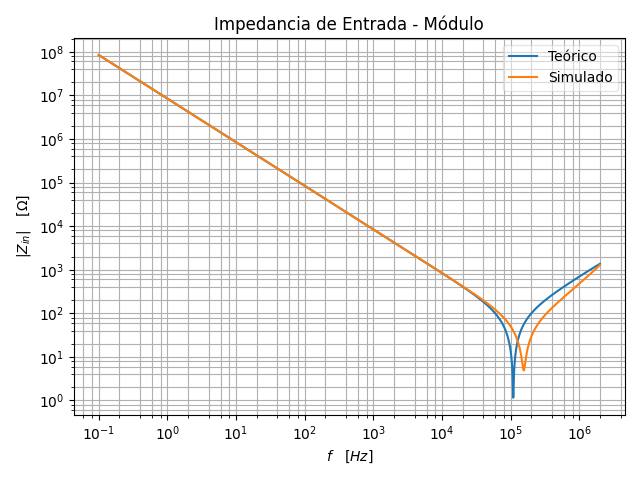
\includegraphics[width=0.6\textwidth]{../Ejercicio3-CircuitoIntegradoresyDerivadores/Imagenes/Derivador/Zin/Z_in_comparacion_mod.png}
    \caption{Comparación Impedancias de entrada - Módulo}
    \label{graph_z_in_mag}
\end{figure}
\begin{figure}[H]
    \centering
    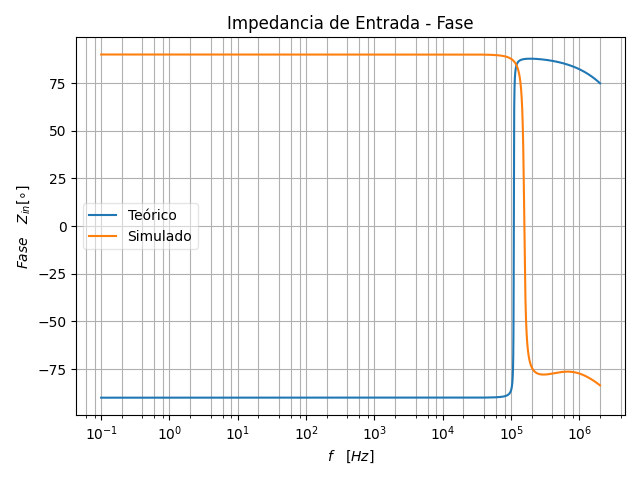
\includegraphics[width=0.6\textwidth]{../Ejercicio3-CircuitoIntegradoresyDerivadores/Imagenes/Derivador/Zin/Z_in_comparacion_pha.png}
    \caption{Comparación Impedancias de entrada - Fase}
    \label{graph_z_in_pha}
\end{figure}
Observando las figuras anteriores, se puede observar una correcta correlación entre la impedancia de entrada 
y las transferencias obtenidas vistas en \ref{graph_trans_mag} y \ref{graph_trans_pha}. Al ponerse el capacitor
en corto alrededor de los $150KHZ$ ocurre el mínimo de impedancia, se observa la coincidencia de sobrepico 
en el gráfico de transferencia. Por otro lado, el sobrepico menos abrupto se debe a que el modelo 
simulado del capacitor contiene una resistencia serie o paralela que no permite que su impedancia se haga
realmente nula.

\subsubsection{Respuesta ante una senoidal}
A continuación, previo al análisis de la respuesta del circuito ante una senoidal, se hace una análisis de las 
frecuencias de operación del circuito que servirán como base para posteriores análisis. \par 
Como primer consideración, se puede afirmar que el comportamiento como derivador, la zona de estudio sobre 
la cual hay interés, coincide para los tres modelos propuestos, por lo tanto, se toma el modelo más sencillo 
 de transferencia dado por \ref{trans_ideal}, considerando un $A_{vol}$ infinito. En dicho caso, el modulo
de la transferencia será proporcional a la frecuencia, estando dado por:
\vspace{2mm}
\begin{equation}
    |H(f)|=\frac{CRf}{2\pi}
    \label{frec_unitaria}
\end{equation}
\vspace{2mm}

Despejando de la función transferencia \ref{trans_ideal} se puede observar que la frecuencia de ganancia 
unitaria del circuito está dada por: 

\vspace{2mm}
\begin{equation}
    f_t=\frac{1}{2\pi RC} \approx 1.6KHz
    \label{frec_unitaria}
\end{equation}
\vspace{2mm}

Dicho valor coincide con el observable en el gráfico \ref{graph_trans_mag}. \par 
Por debajo de $f_t$ se podrán lograr atenuaciones de hasta $50dB$ a frecuencias bajas y ganancias de hasta 
$40dB$ justo antes del polo dominante del circuito, punto en el cual el derivador deja de cumplir su función. \par 
Habiendo realizado todas las consideraciones anteriores, se analiza la respuesta del sistema ante una señal senoidal
de frecuencia $1.6HKz$, esperando observar su comportamiento derivador con una ganancia unitaria.

\begin{figure}[H]
    \centering
    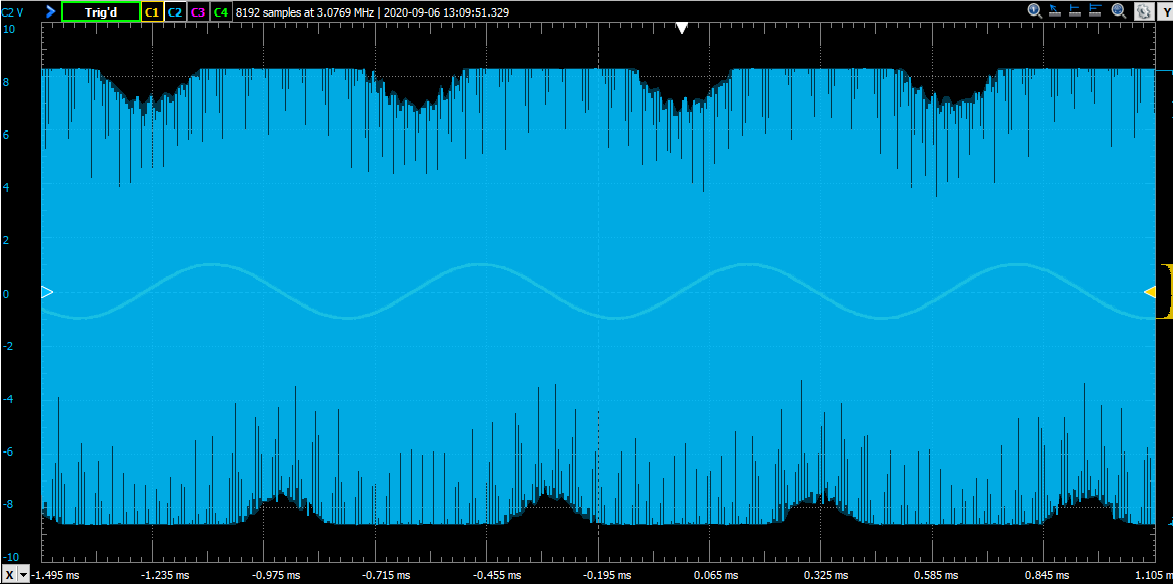
\includegraphics[width=0.6\textwidth]{../Ejercicio3-CircuitoIntegradoresyDerivadores/Imagenes/Derivador/ruido_alto_f.png}
    \caption{Ruido de alta frecuencia generado por el THD del generador}
    \label{thd}
\end{figure}
Lamentablemente, no se observa lo esperado debido a que la experiencia empírica dista en gran medida del modelo 
teórico, esto se debe a factores y limitaciones que no estamos considerando. Para este caso en particular, 
lo que está sucediendo es que el generador de funciones del equipo no es un generador ideal,
 siendo incapaz de ofrecer 
una señal que sólo tenga componentes en la frecuencia deseada, poseyendo una composición armónica
 parásita denominada distorsión armónica
\textit{(THD)}. Para este caso en particular, la THD del generador es alta. \par 
 Los componentes parásitos de alta frecuencia de la señal se ven amplificados según 
la transferencia vista en \ref{graph_trans_mag}, dicho análisis coincide con el visto mediante en el analizador 
de espectro del equipo en el siguiente gráfico. 
\begin{figure}[H]
    \centering
    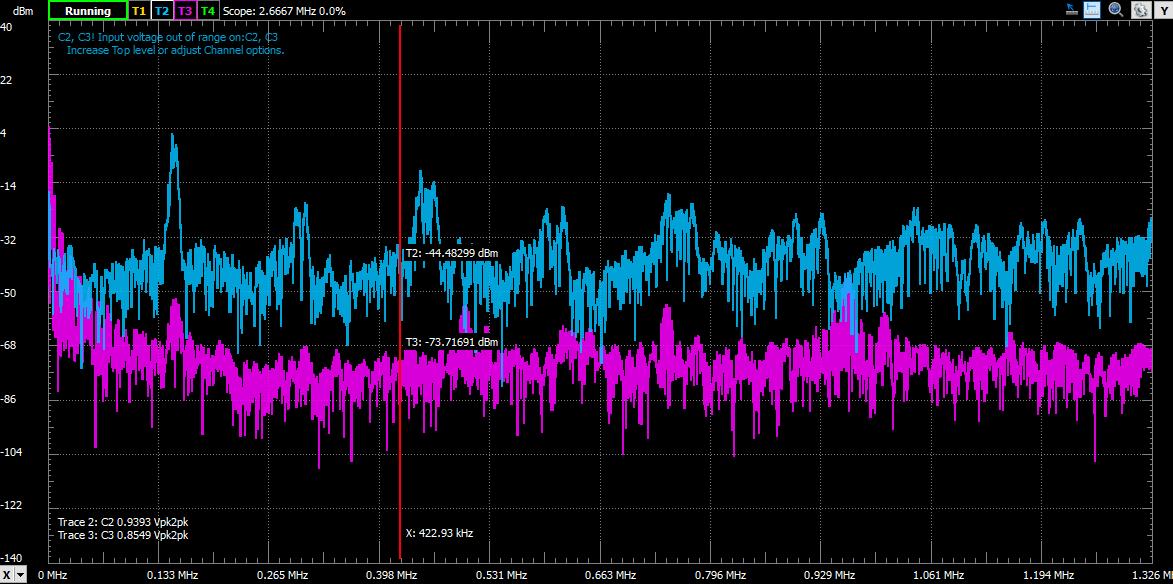
\includegraphics[width=0.6\textwidth]{../Ejercicio3-CircuitoIntegradoresyDerivadores/Imagenes/Derivador/thd.png}
    \caption{Análisis espectral del THD}

\end{figure}
La señal azul es la observada en la salida del derivador mientras que la violeta es su correlativa a la entrada.
A simple vista, los componentes parásitos de la señal de entrada no son distinguibles del piso de ruido, sin embargo
para valores cercanos al pico de transferencia se produce una gran amplificación de los mismos, generando el ruido
observado en  \ref{thd}. \par 
Por ende, para resolver este problema se utiliza un filtro pasa-bajos a la entrada para filtrar los componentes 
parásitos de alta frecuencia provistos por la fuente.  El sistema de medición utilizado es el siguiente:

\begin{figure}[H]
    \centering
    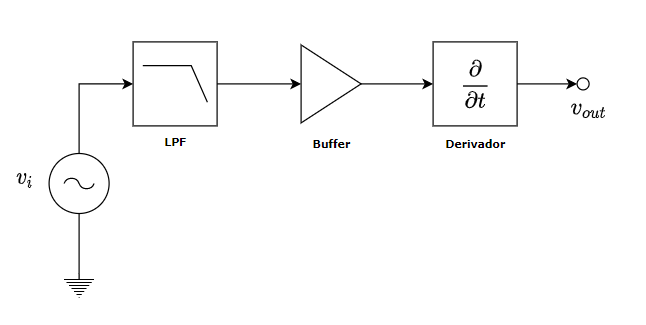
\includegraphics[width=0.6\textwidth]{../Ejercicio3-CircuitoIntegradoresyDerivadores/Imagenes/Derivador/circuito_thd.png}
    \caption{Circuito implementado para reducir el ruido}

\end{figure}
La frecuencia de corte será una década por encima de la frecuencia de la senoidal buscada, en este caso $16KHz$. 
Por otro lado,
habrá que tener en consideración el desfasaje agregado de $-90^\circ$. \par 
Implementado este sistema, se puede observar lo siguiente:

\begin{figure}[H]
    \centering
    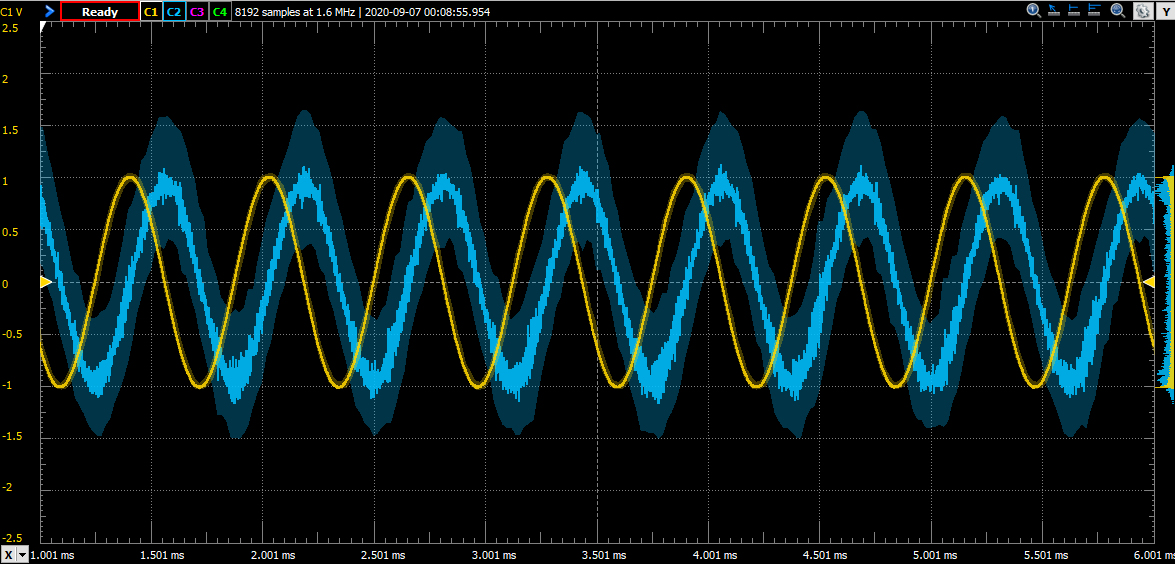
\includegraphics[width=0.6\textwidth]{../Ejercicio3-CircuitoIntegradoresyDerivadores/Imagenes/Derivador/captura_sen.png}
    \caption{Respuesta medida del sistema ante una señal senoidal de 1K6 Hz}

\end{figure}

A continuación, se grafica la comparación entre el la respuesta del sistema 
teórico, medido y simulado.
\begin{figure}[H]
    \centering
    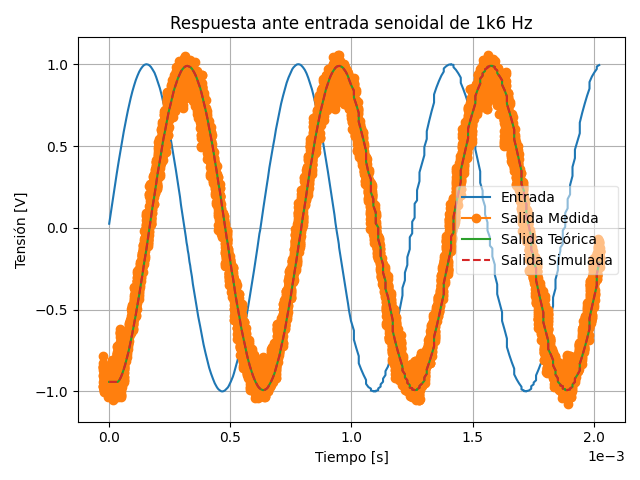
\includegraphics[width=0.6\textwidth]{../Ejercicio3-CircuitoIntegradoresyDerivadores/Imagenes/Derivador/rta_sen_1k6.png}
    \caption{Comparación de la respuesta del sistema ante una señal senoidal de 1K6 Hz}

\end{figure}
Se puede apreciar una excelente correlación entre los tres sistemas planteados.

Para continuar con el análisis del derivador implementado, se estudiará
la respuesta del sistema ante una señal triangular. Para este caso,
se elimina el filtro pasa-bajos ya que deformaría en gran medida 
la señal de la entrada. \par 
Como primer análisis, se elige una señal de amplitud $1V$ y frecuencia 
$1.6 KHz$, la misma coincide con su frecuencia de ganancia unitaria por lo que
se esperará que la señal de salida no vea modificada su amplitud. De otra manera,
lo que si se verá modificado será la forma de la señal, esperando obtener
una señal cuadrada a la salida.

\begin{figure}[H]
    \centering
    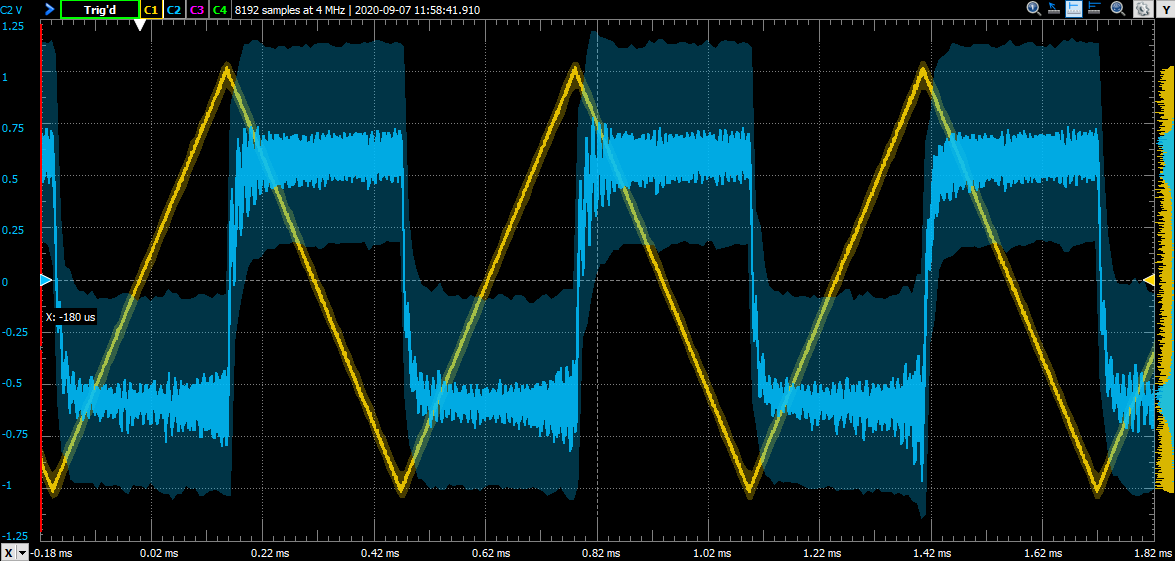
\includegraphics[width=0.6\textwidth]{../Ejercicio3-CircuitoIntegradoresyDerivadores/Imagenes/Derivador/trian_1k6.png}
    \caption{Respuesta medida del sistema ante una señal triangular de 1K6 Hz}

\end{figure}
Teniendo en consideración lo observado en la imagen anterior, se puede sostener que se obtiene 
lo esperado, una señal cuadrada de igual magnitud. El gran nivel de ruido se debe a la presencia 
de componentes de alta frecuencia de la  triangular que son amplificados por el derivador. 

\begin{figure}[H]
    \centering
    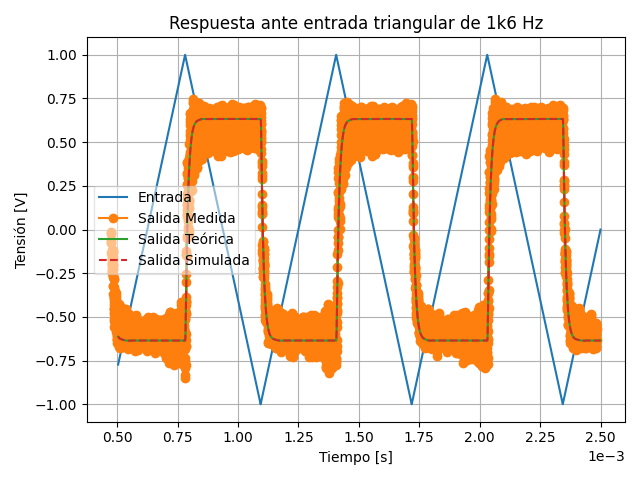
\includegraphics[width=0.6\textwidth]{../Ejercicio3-CircuitoIntegradoresyDerivadores/Imagenes/Derivador/rta_triangular_1k6.png}
    \caption{Comparación de la respuesta del sistema ante una señal triangular de 1K6 Hz}

\end{figure}

El siguiente caso a analizar es el de una señal triangular de amplitud de $1V$, pero con una frecuencia
que se encuentra una década por debajo de la frecuencia de ganancia unitaria, es decir, utilizaremos
una frecuencia de $160Hz$. Observando el gráfico de transferencia visto en \ref{graph_trans_mag}, es
de esperar una atenuación de $20dB$ en la señal de salida.

\begin{figure}[H]
    \centering
    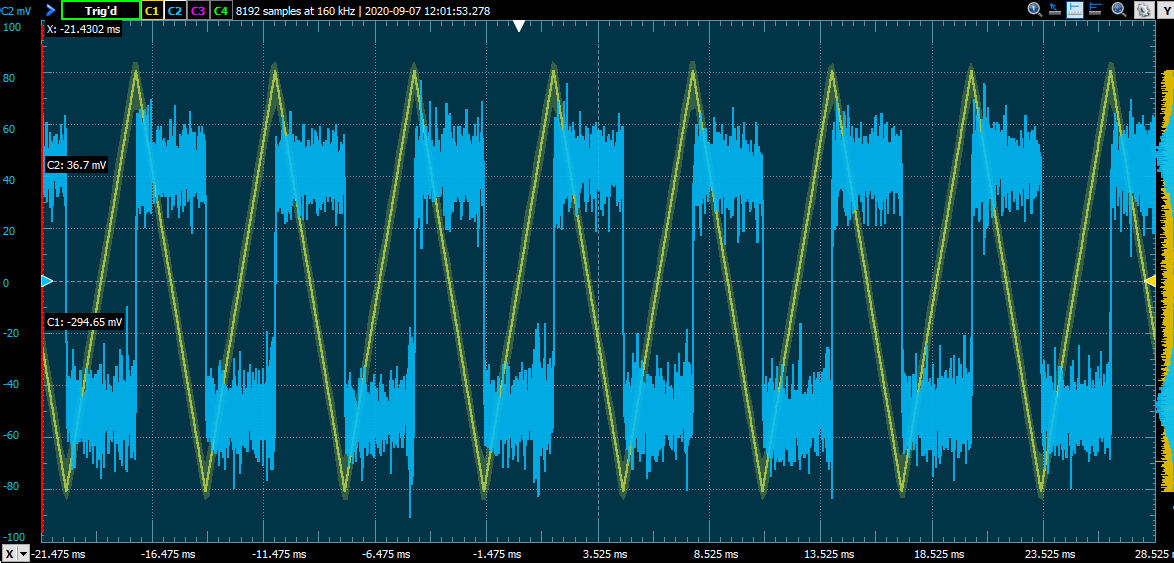
\includegraphics[width=0.6\textwidth]{../Ejercicio3-CircuitoIntegradoresyDerivadores/Imagenes/Derivador/trian_160.png}
    \caption{Respuesta medida del sistema ante una señal triangular de 160 Hz}
\end{figure}
La salida coincide con lo esperado, siendo una señal cuadrada de amplitud $100mV$. Por otro lado,
también se observa un mayor nivel de ruido, esto se debe a que el piso de ruido de alta frecuencia 
se hace más notorio al trabajar con amplitudes más pequeñas.
\begin{figure}[H]
    \centering
    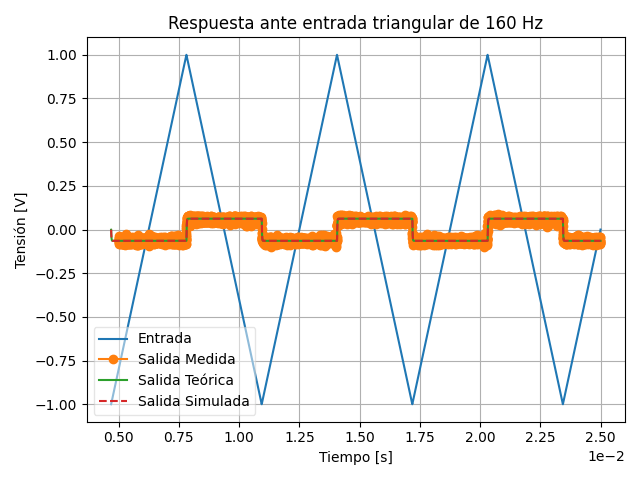
\includegraphics[width=0.6\textwidth]{../Ejercicio3-CircuitoIntegradoresyDerivadores/Imagenes/Derivador/rta_triangular_160.png}
    \caption{Comparación de la respuesta del sistema ante una señal triangular de 160 Hz}

\end{figure}


\subsubsection{Compensación}
En este apartado se realizará un análisis sobre la colocación de una resistencia de compensación
$R_C$ en el circuito para mejorar su funcionamiento, atenuando el sobrepico presente a altas 
frecuencias, alrededor de los $150 KHz$. \par 
Como se puede observar en las gráficas 
ya presentadas de $Z_{in}$ y $H(\$)$ (\ref{graph_trans_mag} y \ref{graph_z_in_mag}), el sobrepico
se debe a que la impedancia del capacitor se vuelve mínima, siendo equivalente a un cortocircuito, de
esta manera, la impedancia de entrada se hace casi cero, permitiendo una transferencia extremadamente alta.\par 
Para corregir dicho inconveniente, es necesario colocar una resistencia de bajo valor 
en serie con el capacitor del circuito 
mostrado previamente en \ref{circuito_medidor_derivador}. De esta manera, cuando la impedancia del capacitor
baje llegará un punto en el que la misma se haga del orden de la resistencia, evitando la situación de cortocircuito
y el sobrepico. Para este punto, el circuito se comportará como un inversor. \par 
Cuando nos referimos a bajo valor hacemos referencia a un valor tal que no afecte el funcionamiento 
normal del derivador, ya sea modificando su transferencia y/o impedancia de entrada. Para calcular el 
valor de resistencia a colocar, se analiza la impedancia del capacitor a dicha frecuencia, siendo la misma:
\vspace{2mm}
\begin{equation*}
    X_c=\frac{1}{2\pi*80KHz**18.88nF}\approx 100 \Omega
\end{equation*}
\vspace{2mm}
Basándonos en el razonamiento anterior, se utilizará una resistencia $R_C$ en serie con 
el capacitor del sistema de valor nominal $100\Omega$. \par 

Los resultados experimentales se presentan a continuación:

\begin{figure}[H]
    \centering
    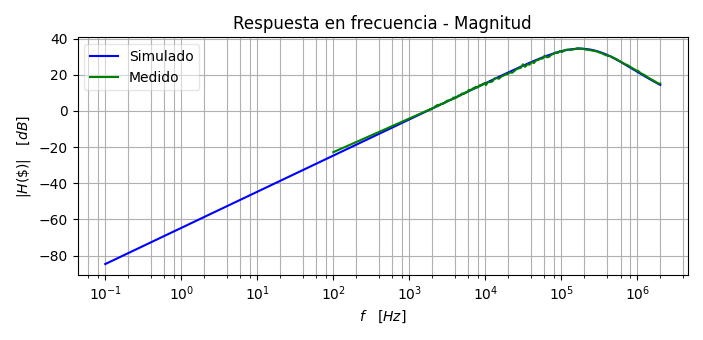
\includegraphics[width=0.6\textwidth]{../Ejercicio3-CircuitoIntegradoresyDerivadores/Imagenes/Derivador/trans_compensa_mag.png}
    \caption{Transferencia compensada - Diagrama de magnitud}

\end{figure}\begin{figure}[H]
    \centering
    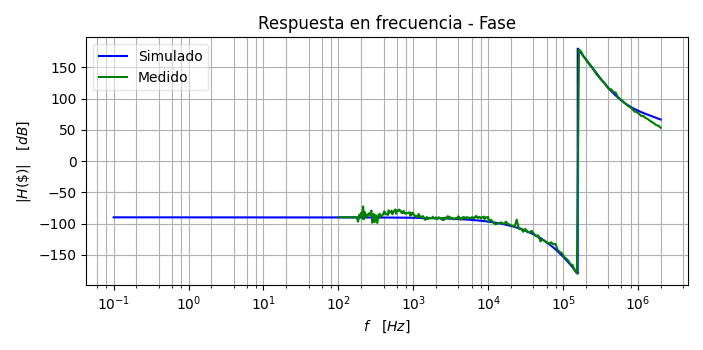
\includegraphics[width=0.6\textwidth]{../Ejercicio3-CircuitoIntegradoresyDerivadores/Imagenes/Derivador/trans_compensa_pha.png}
    \caption{Transferencia compensada - Diagrama de fase}

\end{figure}
Como es de esperar, la transferencia compensada medida coincide con la simulada para nuestro modelo de amplificador 
operacional. Consiguientemente, se procede a comparar los dos sistemas, con y sin compensación.
\begin{figure}[H]
    \centering
    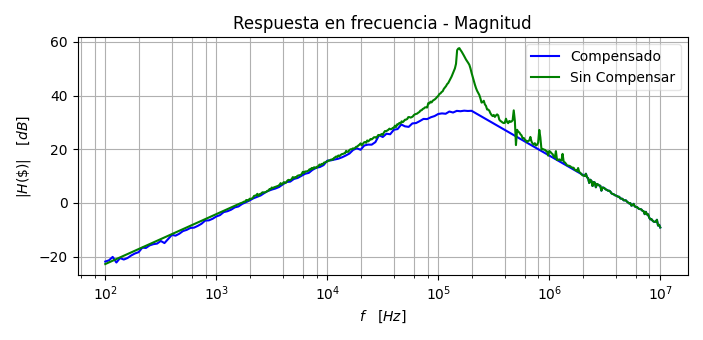
\includegraphics[width=0.6\textwidth]{../Ejercicio3-CircuitoIntegradoresyDerivadores/Imagenes/Derivador/trans_compensa__comp_mag.png}
    \caption{Comparación de las transferencias - Diagrama de magnitud}

\end{figure}\begin{figure}[H]
    \centering
    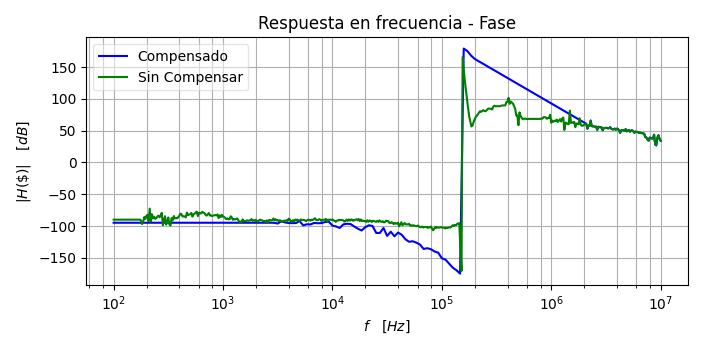
\includegraphics[width=0.6\textwidth]{../Ejercicio3-CircuitoIntegradoresyDerivadores/Imagenes/Derivador/trans_compensa__comp_pha.png}
    \caption{Comparación de las transferencias - Diagrama de fase}

\end{figure}
Como conclusión, se puede afirmar que la compensación se produjo con éxito, teniendo como 
resultado un sistema con menor sobrepico, produciéndose una atenuación de aproximadamente
$30dB$ para dicha frecuencia, otorgandole a la respuesta en frecuencia del circuito mayor 
estabilidad. Por otro lado, el agregado 
de la $R_C$ no modifica la transferencia del circuito original, comportándose de igual manera 
a frecuencias menores a los $150KHz$, zona de interés para el uso de nuestro derivador. \par 
Respecto a la fase, no se observan cambio alguno en la fase de ambos sistemas respecto a la frecuencia para 
la cual el desfasaje es $90^\circ$. Sin embargo, la presencia de $R_C$ suaviza el cambio de fase respecto a los
valores medidos en su ausencia.







\subsection{Circuito Integrador}

\subsubsection{Introducción}

Se realizó el análisis de un circuito integrador ideal, utilizando en este caso tres componentes, una Resistencia $R$,
un capacitor $C$ y un amplificador operacional. 
Cabe destacar que se considera un integrador ideal ya que a diferencia del circuito RC analizado en el primer trabajo práctico de laboratorio,
éste funcionará como integrador para cualquier frecuencia y no solo a frecuencias altas. 

Los valores nominales utilizados para la experiencia fueron:

\begin{itemize}
	\item $R: 5.1K \Omega$ 
	\item $C: 20nF$
	\item $OPAMP: LM833$
\end{itemize}

\begin{figure}[H]
    \centering 
    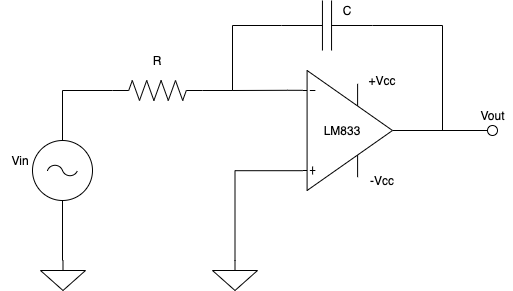
\includegraphics [scale=0.5] {../Ejercicio3-CircuitoIntegradoresyDerivadores/Imagenes/diagrama-integrador.png} 
    \caption{Diagrama del circuito integrador ideal empleado}
    \label{fig:emptyPlotTool}
\end{figure}

A continuación se procederá a calcular teóricamente el valor de las funciones transferencias para los casos en 
donde el amplificador operacional tiene un comportamiento ideal, con $A_{vol}$ finito y $A_{vol}(w)$ con polo dominante.

\subsubsection{Análisis de la Transferencia del Circuito Integrador - OPAMP ideal}

Para obtener la función transferencia en este caso, $H(S) = \frac{V_{out} (S)}{V_{in} (S)}$, partiremos de las siguientes condiciones
iniciales para el amplificador operacional:

\begin{itemize}
	\item $A_{vol}: \infty$
	\item $Z_{in}: \infty$
	\item $Z_{out}: 0$
\end{itemize}

\begin{figure}[H]
    \centering 
    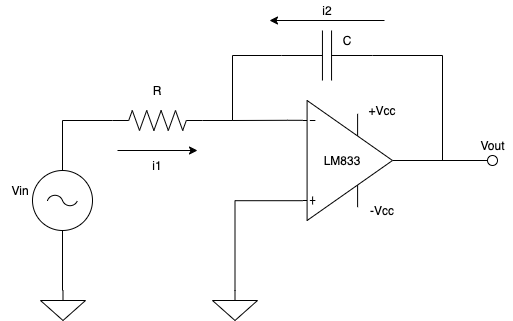
\includegraphics [scale=0.5] {../Ejercicio3-CircuitoIntegradoresyDerivadores/Imagenes/diagrama-integrador-corrientes.png} 
    \caption{Diagrama del circuito integrador ideal empleado}
    \label{fig:emptyPlotTool}
\end{figure}

Podemos observar a simple vista que:

\begin{itemize}
	\item $i1 = -i2$
	\item $i1 = \frac {V_{in}-V^{-}}{R} $
	\item $i2 = \frac {V_{out}-V^{-}}{X_c}$
	\item $V_{out} = A_{vol}(V^{+}-V^{-})$
\end{itemize}

Como ${A_{vol} \to \infty}$ y $V_{out}$ es finito, ${(V^{+}-V^{-}) \to 0}$ y como $V^{+}$ está conectado a tierra,
$(V^{-}$ representa tierra virtual, por lo cual su valor es de $0V$.

Entonces, redefiniendo las ecuaciones anteriores:

\begin{itemize}
	\item $i1 = \frac{V_{in}}{R} $
	\item $i2 = \frac {V_{out}}{X_c}$
\end{itemize}

Siendo entonces:

$$ \frac{V_{in}}{R} = - (\frac{V_{out}}{X_c}) \Longrightarrow \frac{V_{out}}{V_{in}} = -\frac{X_c}{R} = - \frac{1}{SRC}$$

$$ H(S) = - \frac{1}{SRC}$$

Claramente se puede apreciar que este circuito se comportará como un integrador, ya que si antitransformamos la función de transferencia
obtenida implicará que para obtener $v_{out}(t)$ habrá que integrar $v_{in}(t)$ en el dominio del tiempo.

En las siguientes figuras, se puede apreciar el Diagrama de Bode para este caso.

\begin{figure}[H]
    \centering 
    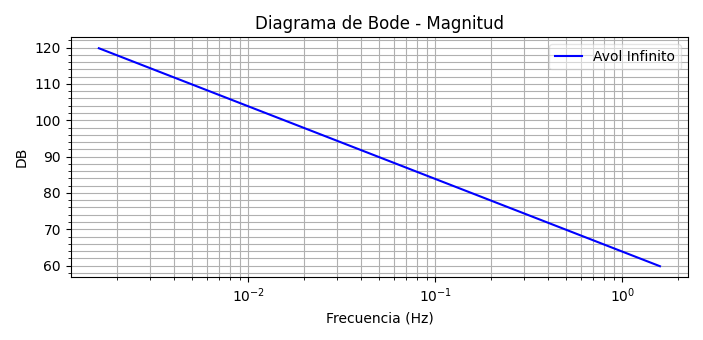
\includegraphics [scale=1] {../Ejercicio3-CircuitoIntegradoresyDerivadores/Imagenes/diagrama-bode-ideal-amplitud.png} 
    \caption{Diagrama de BODE de Amplitud para OPAMP ideal}
    \label{fig:emptyPlotTool}
\end{figure}

\begin{figure}[H]
    \centering 
    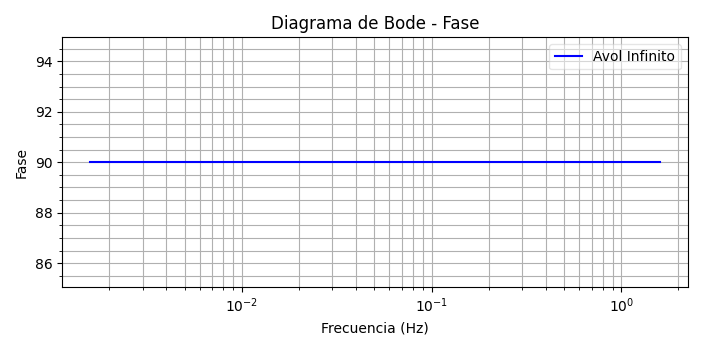
\includegraphics [scale=1] {../Ejercicio3-CircuitoIntegradoresyDerivadores/Imagenes/diagrama-bode-ideal-fase.png} 
    \caption{Diagrama de BODE de Fase para OPAMP ideal}
    \label{fig:emptyPlotTool}
\end{figure}

\subsubsection{Análisis de la Transferencia del Circuito Integrador - OPAMP con A finito}

A diferencia del caso anterior, aquí la diferencia en el cálculo de la función transferencia, $H(S) = \frac{V_{out} (S)}{V_{in} (S)}$,
entre el amplificador operaciones ideal y éste será:

\begin{itemize}
	\item $A_{vol}: finito$
\end{itemize}

Utilizando las mismas relaciones mencionadas en el apartado anterior, podemos observar ahora que:


$$V_{out}=-A_{vol}.V^{-} \Longrightarrow V^{-} = \frac{-V_{out}}{A_{vol}}$$ 


Por lo tanto:

\begin{itemize}
	\item $i1 = \frac {V_{in}-V^{-}}{R} =  \frac {V_{in} + \frac{V_{out}}{A_{vol}}}{R}$
	\item $i2 = \frac {V_{out}-V^{-}}{X_c} = \frac {V_{out} + \frac{V_{out}}{A_{vol}}}{X_c}$
\end{itemize}

Siendo entonces:

$$ \frac {V_{in} + \frac{V_{out}}{A_{vol}}}{R} = -(\frac {V_{out} + \frac{V_{out}}{A_{vol}}}{X_c})
\Longrightarrow \frac{V_{out}}{V_{in}} = \frac{1}{SCR(1+\frac{1}{A_{vol}}+\frac{1}{A_{vol}SRC})}$$

Finalmente:

$$H(S)= \frac{1}{SCR(1+\frac{1}{A_{vol}})+\frac{1}{A_{vol}}}$$

Es importante notar que siendo la ganancia para el caso ideal (GI) $- \frac{1}{SRC}$,  la funcion
transferencia se puede representar como $H(S) = GI. \frac{1}{SCR(1+\frac{1}{A_{vol}})+\frac{1}{A_{vol}}}$
Si $A_{vol}$ es lo suficientemente grande, tendremos una función transferencia ideal nuevamente.

\begin{figure}[H]
    \centering 
    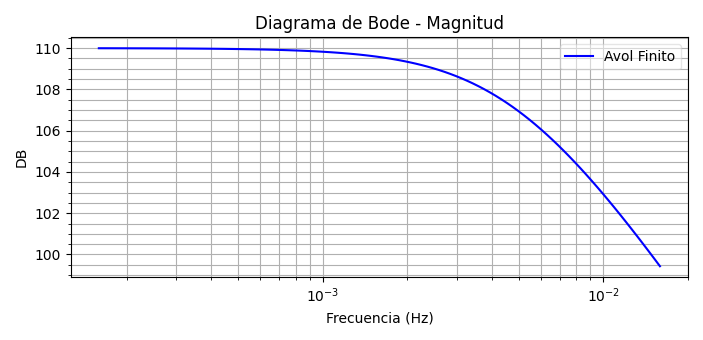
\includegraphics [scale=1] {../Ejercicio3-CircuitoIntegradoresyDerivadores/Imagenes/diagrama-bode-cideal-amplitud.png} 
    \caption{Diagrama de BODE de Amplitud para OPAMP con $A_{vol}$ finito}
    \label{fig:emptyPlotTool}
\end{figure}

\begin{figure}[H]
    \centering 
    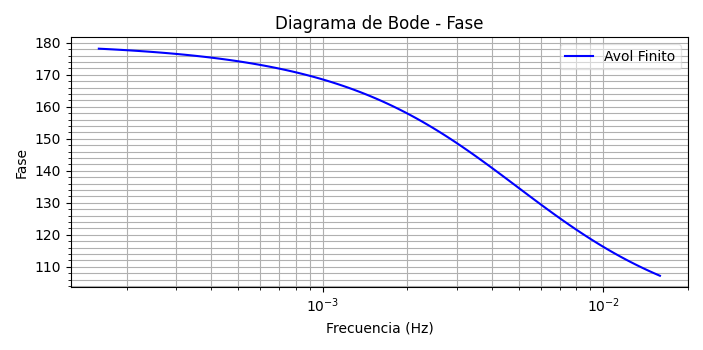
\includegraphics [scale=1] {../Ejercicio3-CircuitoIntegradoresyDerivadores/Imagenes/diagrama-bode-cideal-fase.png} 
    \caption{Diagrama de BODE de Fase para OPAMP con $A_{vol}$ finito}
    \label{fig:emptyPlotTool}
\end{figure}

\subsubsection{Análisis de la Transferencia del Circuito Integrador - OPAMP con $A_{vol}(w)$}

En este ultimo caso de analisis, $A_{vol}$ no es constante sino que es función de la frecuencia según:

$$A_{vol}=\frac{A_0}{1+\frac{S}{w_b}}$$

Por lo cual la expresion para la funcion transferencia calculada en el caso anterior, quedara denominada por:

$$H(S)= \frac{1}{SCR(1+\frac{1+\frac{1}{SCR}}{A_{vol}})}\Longrightarrow H(S)= \frac{1}{SCR(1+\frac{1+\frac{1}{SCR}}{\frac{A_0}{1+\frac{S}{w_b}}})}$$ 

Reacomodando algebraicamente:

$$H(S)=- \frac{1}{S^2\frac{CR}{A_oW_b}+SCR(1 + \frac{1}{A_o}+\frac{1}{W_bA_oCR}) + \frac{1}{A_0}}$$

Podemos observar que si $A_o$ es muy grande, nuevamente estaremos en el caso donde la ganancia que obtendremos será la ideal para este circuito.

\begin{figure}[H]
    \centering 
    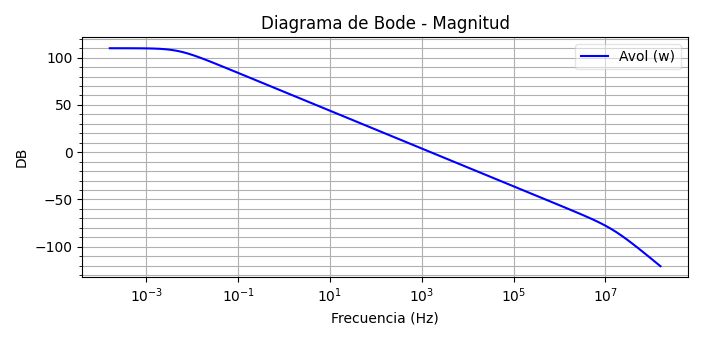
\includegraphics [scale=1] {../Ejercicio3-CircuitoIntegradoresyDerivadores/Imagenes/diagrama-bode-noideal-amplitud.png} 
    \caption{Diagrama de BODE de Amplitud para OPAMP con $A_{vol}(w)$ finito}
    \label{fig:emptyPlotTool}
\end{figure}

\begin{figure}[H]
    \centering 
    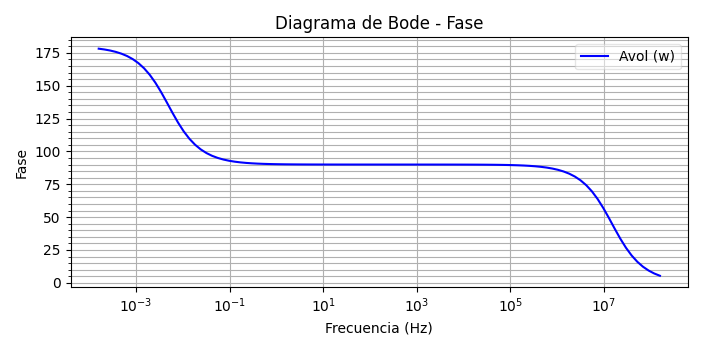
\includegraphics [scale=1] {../Ejercicio3-CircuitoIntegradoresyDerivadores/Imagenes/diagrama-bode-noideal-fase.png} 
    \caption{Diagrama de BODE de Fase para OPAMP con $A_{vol}(w)$ }
    \label{fig:emptyPlotTool}
\end{figure}

Comparando los tres casos, podemos observar que en determinadas frecuencias el comportamiento es identico:

\begin{figure}[H]
    \centering 
    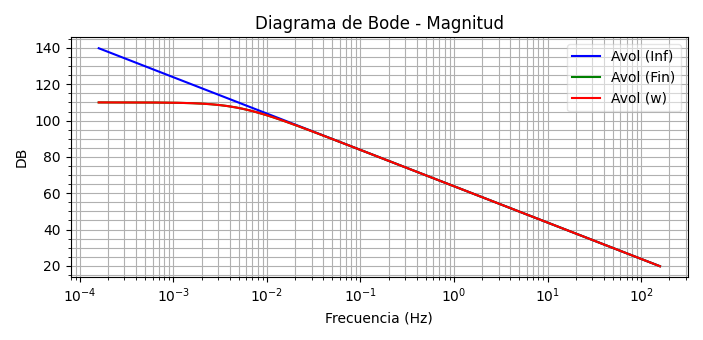
\includegraphics [scale=1] {../Ejercicio3-CircuitoIntegradoresyDerivadores/Imagenes/comparativo-magnitud.png} 
    \caption{Diagrama de BODE de Amplitud para OPAMP comparativo }
    \label{fig:emptyPlotTool}
\end{figure}

\begin{figure}[H]
    \centering 
    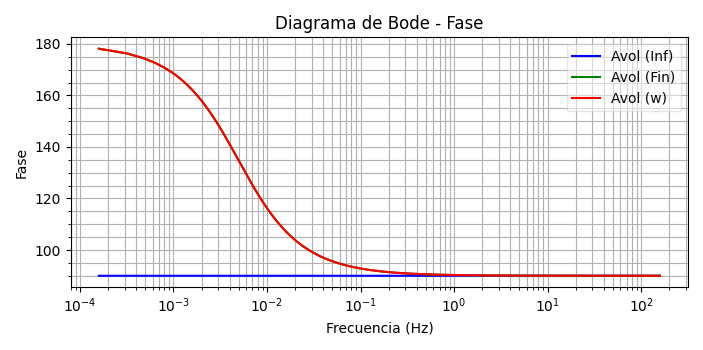
\includegraphics [scale=1] {../Ejercicio3-CircuitoIntegradoresyDerivadores/Imagenes/comparativo-fase.png} 
    \caption{Diagrama de BODE de Fase para OPAMP comparativo }
    \label{fig:emptyPlotTool}
\end{figure}

\subsubsection{Análisis de Impedancia de Entrada al Circuito Integrador}

Para poder calcular teoricamente, la impedancia de entrada, $Z_{in}$, se utilizó el teorema de Miller tal que:

